\documentclass{article}
\usepackage[utf8]{inputenc}
\usepackage[spanish]{babel}
\usepackage{listings}
\usepackage{graphicx}
\graphicspath{ {images/} }
\usepackage{cite}

\begin{document}

\begin{titlepage}
    \begin{center}
        \vspace*{1cm}
            
        \Huge
        \textbf{Parcial 1 (15\%)}
            
        \vspace{0.5cm}
        \LARGE
        Calistenia
        \vspace{0.5cm}
        
        Enlace al video de YouTube con la evidencia: \href{https://youtu.be/fs0ttvP09yI}
            
        \vspace{1.5cm}
            
        \textbf{Nelson Fernando Parra Guardia}
            
        \vfill
            
        \vspace{0.8cm}
            
        \Large
        Despartamento de Ingeniería Electrónica y Telecomunicaciones\\
        Universidad de Antioquia\\
        Medellín\\
        Marzo de 2021
            
    \end{center}
\end{titlepage}

\newpage

Seleccionar su mano más hábil y realizar los siguientes pasos con esa única mano:
\begin{enumerate}

    \item Levantar la hoja conservando su forma inicial.
    \item Ubicar la hoja de manera horizontal sobre la superficie plana mas cercana a las tarjetas, evitando que la hoja permanezca encima de las cartas nuevamente, y soltar.
    \item Tomar ambas tarjetas (conservando su forma) y cambiarlas a posición vertical (si no lo están) reposando sobre la superficie donde se encuentran.
    \item Posicionar:
    
    \begin{enumerate}
    
        \item Si es una persona diestra: el dedo pulgar sobre la esquina superior izquierda de las tarjetas y el dedo índice sobre la esquina superior derecha de las tarjetas, simultáneamente.
        \item \item Si es una persona zurda: el dedo pulgar sobre la esquina superior derecha de las tarjetas y el dedo índice sobre la esquina superior izquierda de las tarjetas, simultáneamente.
        
    \end{enumerate}
    
    \item En esa posición, agarrar las tarjetas y mantenerlas en posición vertical (formando un ángulo recto con respecto a la superficie donde se ubicaban).
    \item Sin soltarlas, con los dedos posicionados como se describió anteriormente y manteniendo su orientación (vertical con respecto a la superficie plana), hacer que las tarjetas estén en contacto, lo más centrado posible, con la hoja de papel previamente reubicada.
    \item En la Figura (\ref{fig:fingers}), se presenta el nombre de los dedos de la mano como guía. Sin soltar en ningún momento las tarjetas:
    
    \begin{enumerate}
    
        \item Si es una persona diestra: con el dedo anular tocar el lateral a su derecha de la tarjeta más próxima a la palma de su mano y con el dedo medio tocar el lateral a su derecha de la tarjeta más alejada a la palma de su mano, empezar a separar lentamente ambas tarjetas para ir formando una pirámide.
        \item Si es una persona zurda: con el dedo anular tocar el lateral a su izquierda de la tarjeta más próxima a la palma de su mano y con el dedo medio tocar el lateral a su izquierda de la tarjeta más alejada a la palma de su mano, empezar a separar lentamente ambas tarjetas para ir formando una pirámide. 
        
    \end{enumerate}

    \begin{figure}[h]
    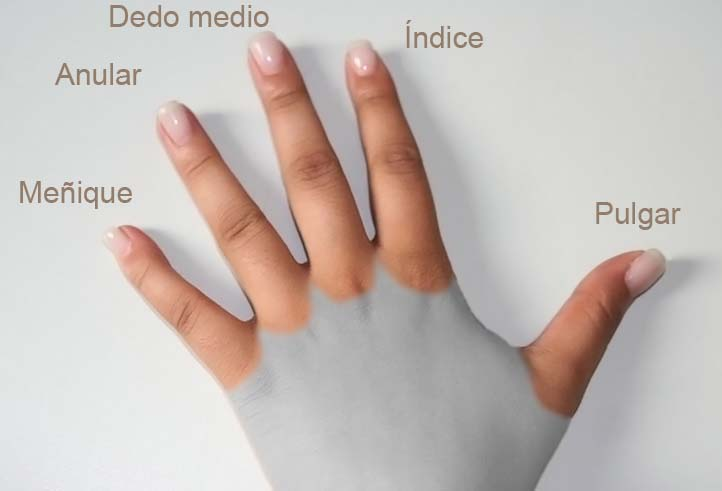
\includegraphics[width=4cm]{fingers.jpg}
    \centering
    \caption{Dedos de la mano.}
    \label{fig:fingers}
    \end{figure}
    
    \item Cuando considere que ambas tarjetas pueden permanecer en posición de pirámide (sin la ayuda de su mano), empiece lentamente a retirar su mano de las tarjetas, hasta soltarlas completamente.
    \item Finalmente, si no permanecen en la posición de pirámide deseada:
    
    \begin{enumerate}
    
        \item Ubicar las tarjetas en su forma inicial (una tarjeta por encima de la otra, en posicion vertical sobre la hoja de papel).
        \item Repetir las instrucciones desde el paso 4.
        
    \end{enumerate}
    
\end{enumerate}

\end{document}
